\documentclass[aps,pra,superscriptaddress,preprint]{revtex4-1}
%\documentclass{article}
\usepackage{amsmath}    % need for subequations
\usepackage{graphicx}   % need for figures
\usepackage[dvipdfx,cmyk]{xcolor}     % use if color is used in text
\usepackage[colorlinks,linkcolor=red,citecolor=brown,urlcolor=blue]{hyperref}
\usepackage{dsfont,bm}
\usepackage{color}
\usepackage{placeins}

% ***********************************************************
% ******************* PHYSICS HEADER ************************
% ***********************************************************
% Version 2
\usepackage{amsmath} % AMS Math Package
\usepackage{amsthm} % Theorem Formatting
\usepackage{amssymb}	% Math symbols such as \mathbb
\usepackage{graphicx} % Allows for eps images
\renewcommand{\labelenumi}{(\alph{enumi})} % Use letters for enumerate
% \DeclareMathOperator{\Sample}{Sample}
\let\vaccent=\v % rename builtin command \v{} to \vaccent{}
\renewcommand{\v}[1]{\ensuremath{\boldsymbol{#1}}} % for vectors
\newcommand{\gv}[1]{\ensuremath{\mbox{\boldmath$ #1 $}}}
% for vectors of Greek letters
\newcommand{\uv}[1]{\ensuremath{\mathbf{\hat{#1}}}} % for unit vector
\newcommand{\abs}[1]{\left| #1 \right|} % for absolute value
\newcommand{\avg}[1]{\left< #1 \right>} % for average
\let\underdot=\d % rename builtin command \d{} to \underdot{}
\renewcommand{\d}[2]{\frac{d #1}{d #2}} % for derivatives
\newcommand{\dd}[2]{\frac{d^2 #1}{d #2^2}} % for double derivatives
\newcommand{\pd}[2]{\frac{\partial #1}{\partial #2}}
% for partial derivatives
\newcommand{\pdd}[2]{\frac{\partial^2 #1}{\partial #2^2}}
% for double partial derivatives
\newcommand{\pdc}[3]{\left( \frac{\partial #1}{\partial #2}
 \right)_{#3}} % for thermodynamic partial derivatives
\newcommand{\ket}[1]{\left| #1 \right>} % for Dirac bras
\newcommand{\bra}[1]{\left< #1 \right|} % for Dirac kets
\newcommand{\proj}[1]{\left| #1 \right>\left< #1 \right|} % for Dirac kets
\newcommand{\braket}[2]{\left< #1 \vphantom{#2} \right|
 \left. #2 \vphantom{#1} \right>} % for Dirac brackets
\newcommand{\matrixel}[3]{\left< #1 \vphantom{#2#3} \right|
 #2 \left| #3 \vphantom{#1#2} \right>} % for Dirac matrix elements
\newcommand{\grad}[1]{\gv{\nabla} #1} % for gradient
\let\divsymb=\div % rename builtin command \div to \divsymb
\renewcommand{\div}[1]{\gv{\nabla} \cdot #1} % for divergence
\newcommand{\curl}[1]{\gv{\nabla} \times #1} % for curl
\let\baraccent=\= % rename builtin command \= to \baraccent
\renewcommand{\=}[1]{\stackrel{#1}{=}} % for putting numbers above =
\newtheorem{prop}{Proposition}
\newtheorem{thm}{Theorem}[section]
\newtheorem{lem}[thm]{Lemma}
\theoremstyle{definition}
\newtheorem{dfn}{Definition}
\theoremstyle{remark}
\newtheorem*{rmk}{Remark}

% ***********************************************************
% ********************** END HEADER *************************
% *********************************************************** 

\graphicspath{{Figures/}}

\begin{document}
\title{Optsimal strategies for generating long-distance entanglement between NV nodes}

\author{Peter C. Humphreys}
\affiliation{Clarendon Laboratory, Department of Physics, University of Oxford, OX1 3PU, United Kingdom}


\begin{abstract}
\end{abstract}
%\maketitle

Blah blah.. Recent progress in the generation, manipulation and storage of distant entangled quantum states has opened up an avenue to the construction of a small-scale quantum network over metropolitan scale distances in the near future. This motivates the exploration of different potential methods for the efficient generation of entangled links between nodes. Here we have examined three different protocols using both semi-analytical and Monte Carlo methods. 

\section{Protocols}

The central challenge for generating entanglement over long distances is the communication overhead required to determine whether entanglement generation succeeded. 

\subsection{Multiplexed Barrett and Kok}

The first scheme that we consider is a version of the Barrett and Kok protocol. In this scheme, entanglement is generated at both nodes between the spin state of the NV and the modal occupation of single photon (typically encoded in the photonic time degree of freedom for NVs). Interfering these single photons on a beamsplitter erases which-path information, allowing entanglement to be generated between the two NV spins, conditional on detecting one output photon in each of the time bins. 

In the standard version of this scheme, the clock rate is limited by the classical communication time required to establish whether the protocol succeeded. For 50 km, this is 250 $\mu$s, limiting the attempt rate of the scheme to 4 kHz.  


\begin{figure}[htbp]
\begin{center}
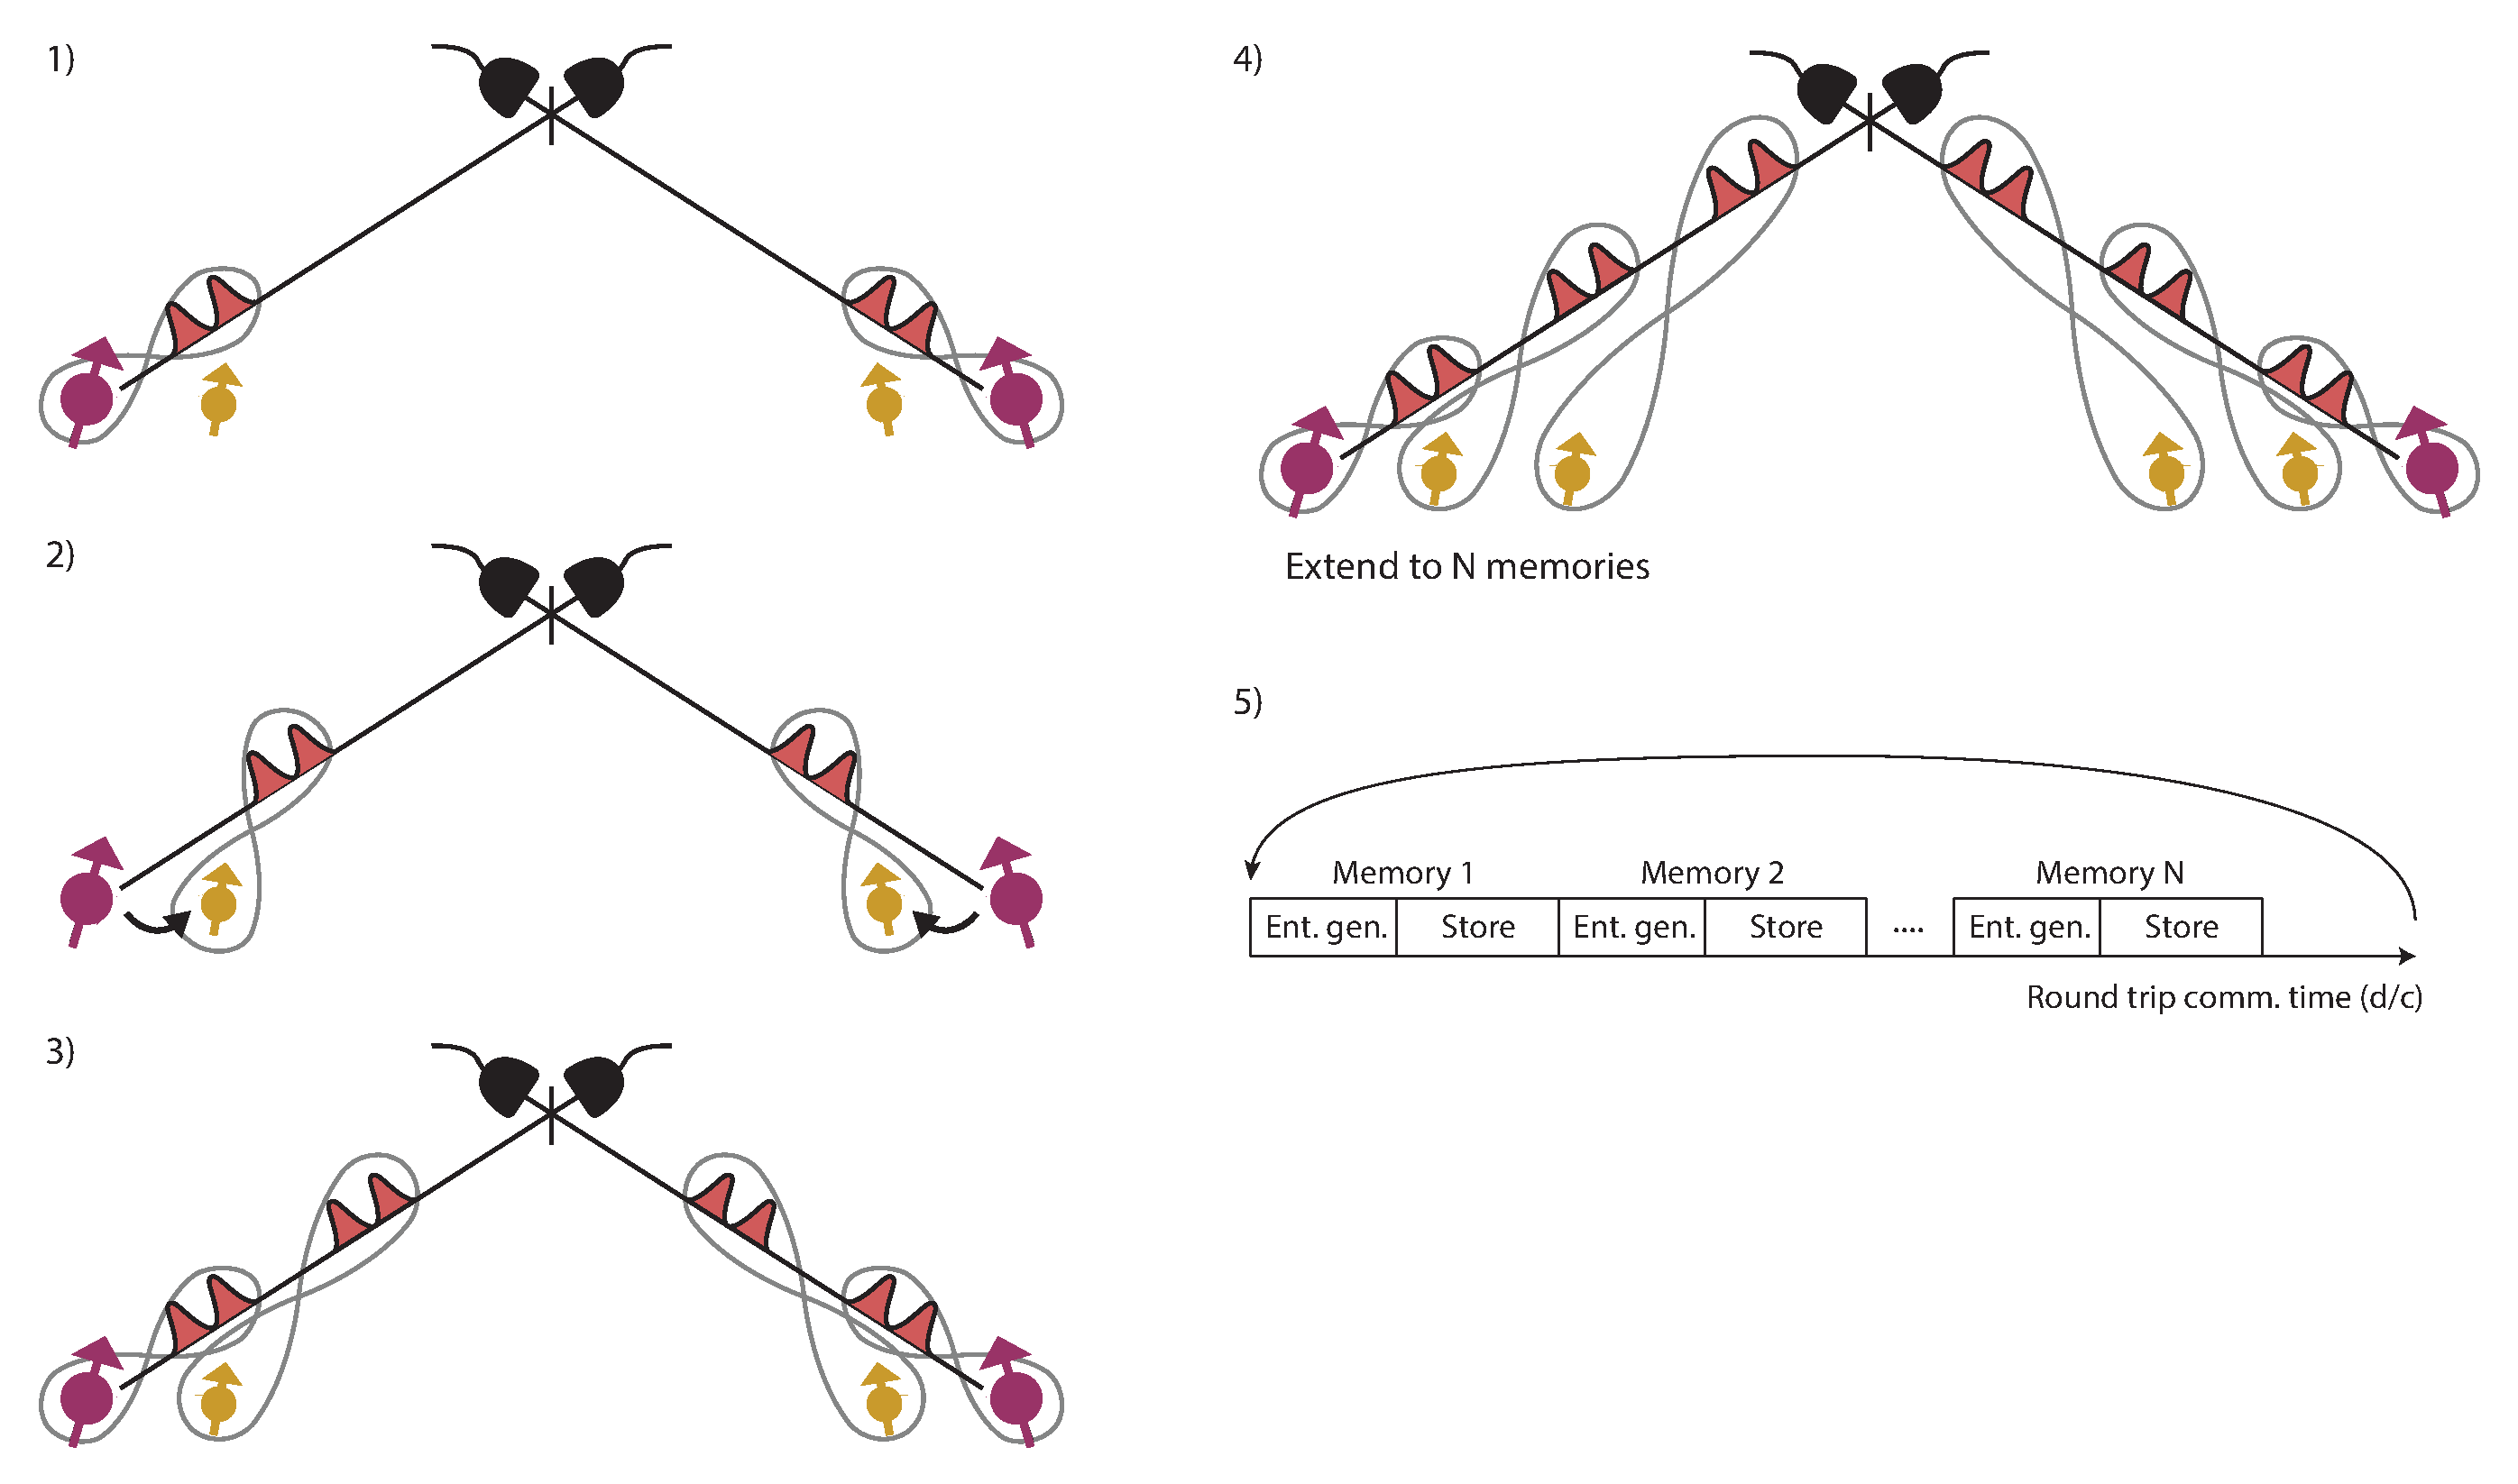
\includegraphics[width=12.0cm]{MultiplexingDiagram.pdf}
\caption{A random figure I started making at some point.}
\label{fig:MultiplexingDiagram}
\end{center}
\end{figure}

\subsection{Multiplexed Extreme Photon Loss Protocol}

\subsection{Kwiat scheme}

\section{Modelling}

\subsection{Parameters}
In our models we have considered two different regimes of parameters, as shown in Table~\ref{tab:Variables}. The `ambitious' regime parameters represent our optimistic expectations for the performance of quantum nodes based on Nitrogen Vacancy (NV) solid-state spins in the medium term (5-10 years), while the `near-term' parameters reflect our expectations for the achievable performance in the shorter term. Both regimes rely on the availability of a cavity system to enhance the ZPL emission of the NV, and on the availability of frequency conversion to convert emitted photons to telecom wavelengths. These technologies are viewed as prerequisites to a scalable quantum network.  

\begin{table}[ht]
\caption{Variables used in these simulations}
\begin{center}
\begin{tabular}{|c|l|c|c|}
\hline
Variable & Description & Ambitious value & Near-term value \\ \hline
$d$ & separation between nodes in km & & \\
$n$ & number of memories (including NV) & 3 & 2 \\
$\eta$ & speed of light in fibre & 0.2 km/$\mu$s & 0.2 km/$\mu$s \\
$\eta$ & fibre attenuation at telecom wavelengths & 0.2 dB/km & 0.2 dB/km \\
$p_\text{fc}$ & frequency conversion efficiency & 0.3 & 0.1 \\
$p_\text{out}$ & NV outcoupling efficiency & 0.3 & 0.1 \\
$t_\text{eg}$ & spin-photon entanglement generation time &1 $\mu$s & 2 $\mu$s\\
$t_\text{cg}$ & NV-carbon gate time  & 10 $\mu$s & 100 $\mu$s \\
$p_m$ & SPDC source photon-pair emission probability  & 0.1 & 0.01 \\ \hline
\end{tabular}
\end{center}
\label{tab:Variables}
\end{table}%

%Probability that a photon will survive over the distance of d/2 km:
%\begin{equation}
%p_\text{loss} = 10^{-\eta d/20}
%\end{equation}
%
%Probability that if one photon got emitted from the NV, it will be collected, successfully converted to telecom and it successfully arrives at the BS:
%\begin{equation}
%p = p_\text{loss} p_\text{fc} p_\text{out}
%\end{equation}

\subsection{Observations}

1) Even for the highly ambitious values, storing in memory takes a long time, comparable to the time required for information to propagate from one node to the other. This limits the number of memories that can be usefully utilised, as can be seen in Fig.~\ref{fig:AmbAndNearValuesRateVsDistance}, in which the dashed red line denotes the distance below which the time required to store states in the memories is longer than the communication time between the nodes. For distances less than this, there is no point in using this number of memories. This is particularly damaging to the Kwiat scheme, since this scheme relies on being able to make many attempts to generate entanglement during one communication cycle.

\begin{figure}[htbp]
\begin{center}
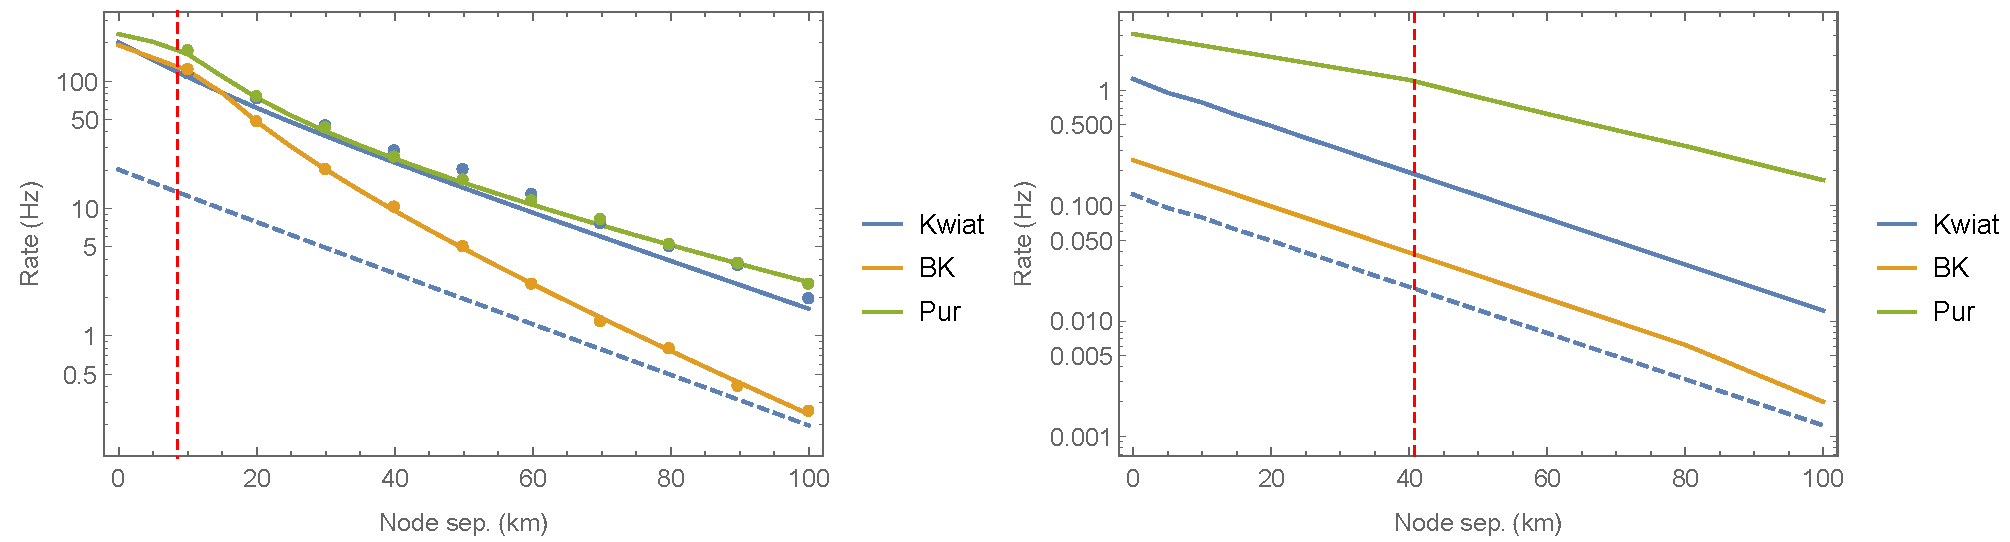
\includegraphics[width=16.0cm]{AmbAndNearValuesRateVsDistance.pdf}
\caption{a) Rate of entanglement generation as a function of distance using different multiplexed schemes with the 'near-term' parameters. For all distances, the multiplexed purification scheme outperforms Barrett and Kok. The effectiveness of the Kwiat scheme is highly dependent on the entangled photon pair generation efficiency. The solid line shows the results for a pair generation probability of 0.1, the dashed line for 0.01. The latter is more consistent with the performance of current sources (some actual research needed on this point). Filled circles show results from Monte Carlo simulations of the same protocols (expected to be more accurate since fewer approximations needed). The vertical red line shows the distance below which all time is used for storing in memories. b) Same plots, for 'ambitious' parameters. For distances greater than 20 km, the multiplexed purification schemes outperform Barrett and Kok.}
\label{fig:AmbAndNearValuesRateVsDistance}
\end{center}
\end{figure}

2) This is apparent when fixing the distance between the nodes and changing the number of available memories. For both the ambitious and the near-term values, the Kwiat scheme derives no benefit from additional memories (in essence, the chance of a successful event in one communication round is very low for both regimes (numbers needed), and so having additional memories with which to store successful events is of no benefit). For the near-term values, there is no benefit for BK or Purification, since, as the red dashed line shows, beyond 2 memories, all time is taken up with storing states. In contrast, for the ambitious values, there is a benefit to increasing the number of memories.

\begin{figure}[htbp]
\begin{center}
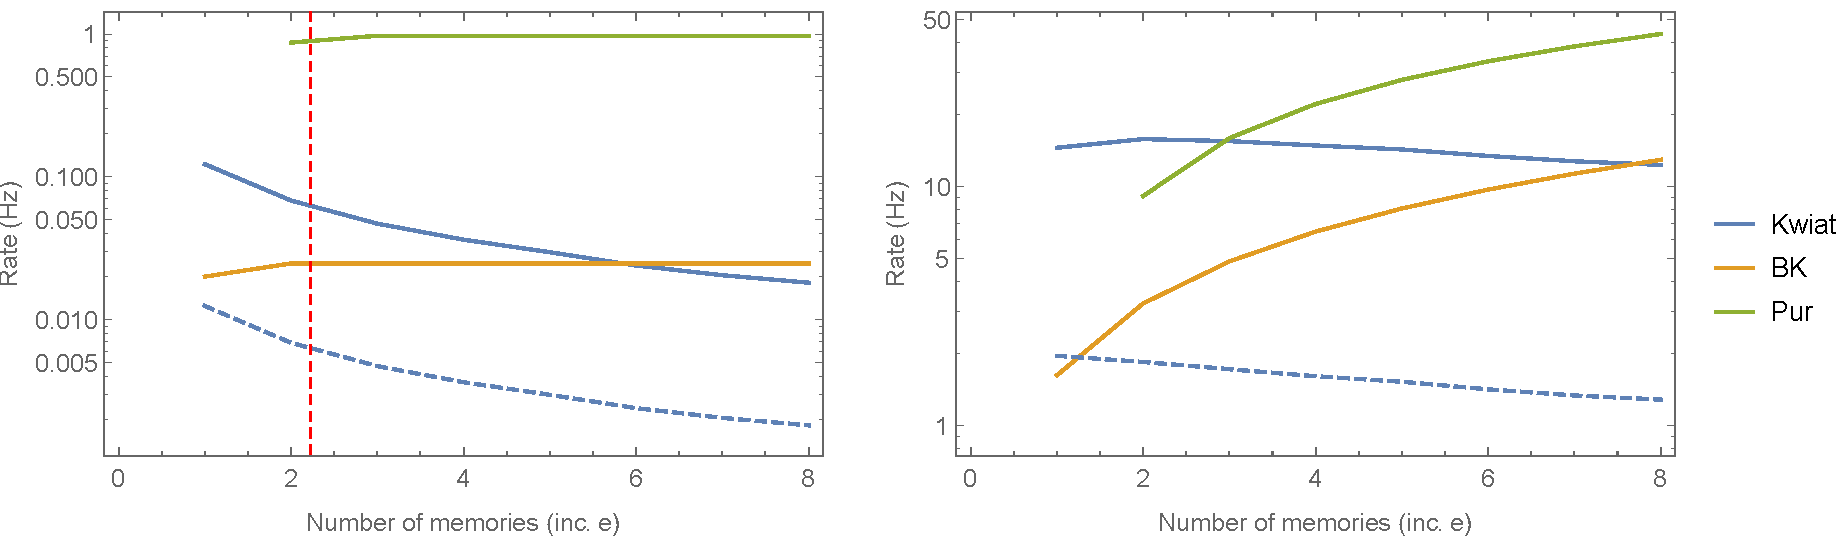
\includegraphics[width=16.0cm]{AmbAndNearValuesRateVsMemories.pdf}
\caption{a) Rate of entanglement generation as a function of number of memories using different multiplexed schemes with the 'near-term' parameters at a fixed distance of 50 km. The vertical red line shows the number of memories beyond which all time is used for storing in memories. b) Same plots, for 'ambitious' parameters.}
\label{fig:AmbAndNearValuesRateVsMemories}
\end{center}
\end{figure}

3) Rate is only half of the story. Changing the parameters also impacts the fidelity of the state produced. In the previous plots, there was no constraint on the minimum acceptable fidelity, and so the rate was maximised. However, in any useful protocol this will not be the case. For a given set of parameters, it is possible to constrain the maximum number of entanglement generation attempts that a given stored state will be subjected to. This will increase the fidelity of the state, at the expense of the entanglement generation rate.

\begin{figure}[htbp]
\begin{center}
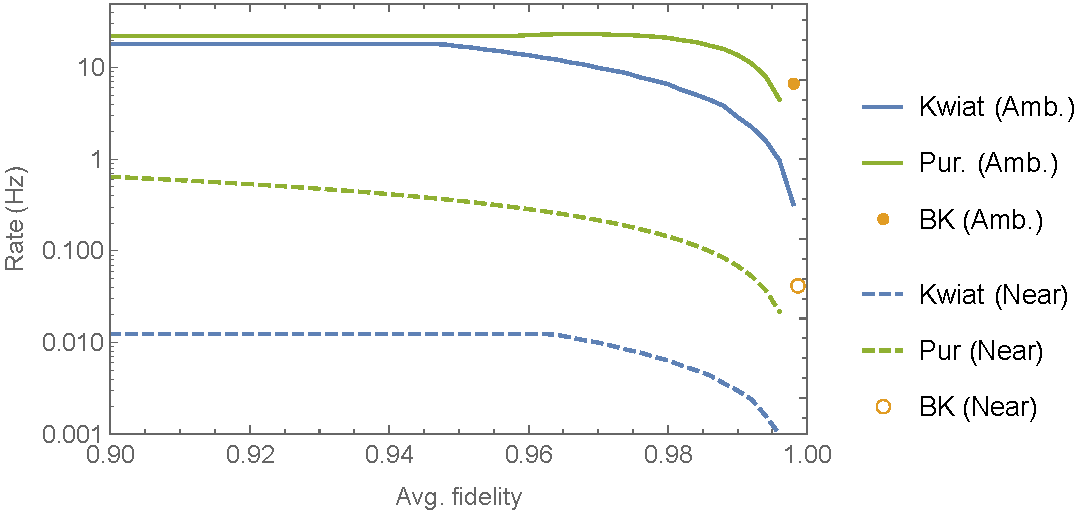
\includegraphics[width=16.0cm]{FidVsRateFixedDistance.pdf}
\caption{By bounding the acceptable average fidelity, it is possible to compromise between the achievable rate and the fidelity. This is shown for a fixed distance of 50 km and a) the 'near-term' parameters, b) the 'ambitious' parameters.}
\label{fig:FidVsRateFixedDistance}
\end{center}
\end{figure}

\end{document}

